\chapter{Helium Interaction with BCC Lithium}
Lithium is becoming one of the important materials in the context of plasma-facing in thermonuclear magnetic fusion devices. Lithium-coated surfaces are being used in several fusion devices in the world~\cite{bell2009plasma, mirnov2003li, sanchez2009impact, tuccillo2009overview, xu2011study, munaretto2012rfx}. There are earlier example of using lithium in the fusion reactor. Erents \etal~\cite{erents1971trapping}\@ used lithium to trap deutorons in solid and liquid lithium. Liquid lithium proven to be efficient trapper. Lithium reacts with deuterium and forms lithium hydride (LiH) which is ionic in nature. Lithium was also proposed as a breeding material in fusion reactors~\cite{hartley1978potential}. For this, lithium needs to be enriched to $^6$Li. The recent interest of using solid lithium (applied to graphite surface) in fusion reactor is for density and impurity control in the temperature range of 30--50 \textdegree C~\cite{allain2012lithium}.  In the near surface of plasma facing materials high density of interstitials and vacancies are being produced in addition to higher concentration of hydrogen and helium. This defects and gases will change the microstructure of the material. It is therefore important to determine the property of point defects in Lithium and its interaction with helium atom. The goal of this study is to calculate some important data regarding point defects in lithium and helium in lithium using first principle methods.

We perform all our calculations using density functional theory (DFT) with plane-wave basis sets as implemented in the software \textsc{QuantumEspresso}\cite{giannozzi2009quantum}. The PAW~\cite{blochl1994projector} based pseudopotential were used from PS library~\cite{dal2014pseudopotentials,pp1}. The generalized gradient approximation of Perdew--Burke--Ernzerhof (PBE) was used as exchange-correlation functional~\cite{Perdew1996b, Perdew1997}. We used a $4\times4\times4$ of bcc lithium, which consists of 128 atoms to simulate point defects. Brillouin zone sampling was performed using Monkhorst and Pack scheme~\cite{pack1977special}. The plane wave cutoff energy was 50 Ry. The equilibrium lattice parameter obtained was 3.436 \AA\@ for bcc lithium. All the calculations were performed at constant volume fully relaxing the atomic positions in the supercells. The migration energies were calculated using the nudged elastic band~\cite{henkelman2000climbing, henkelman2000improved} method with five images along the migration path.

The formation energies are calculated as follows:
\begin{align}\label{eq_forme}
\begin{split}
 E_{f}^{\text{oct}} & = E_{\text{Li}+\text{He}_{\text{oct}}} - E_{\text{Li}_N} - E_{\text{He}_{\text{isolated}}} \\
 E_{f}^{\text{tetr}}& = E_{\text{Li}+\text{He}_{\text{tetr}}} - E_{\text{Li}_N} - E_{\text{He}_{\text{isolated}}} \\
 E_f^{\Box} & = E^{{\Box}_1}_{\text{Li}_{N-1}} - \frac{N-1}{N} E_{\text{Li}_N} \\
 E_f^{\text{subs}} & = E_{\text{Li}+\text{He}_{\Box}} - \frac{N-1}{N} E_{\text{Li}_N} - E_{\text{He}_{\text{isolated}}}
\end{split}
 \end{align}

\nomenclature{$E_f^{\text{subs}}$}{helium formation energy in a substitutional position}
\nomenclature{$E_f^{\text{tetr}}$}{helium formation energy in a tetrahedral position}
\nomenclature{$E_f^{\text{oct}}$}{helium formation energy in a octahedral position}
\nomenclature{$E_{\text{He}_{\text{isolated}}}$}{energy of an isolated helium atom}



Here $E_{\text{Li}+\text{He}_{\text{tetra/octa}}}$ is the energy of the system where He is in either octahedral and tetrahedral location of bcc lithium. $E_{\text{Li}+\text{He}_{\Box}}$ is the energy of the system where He is in substitutional position of the lattice. $E_{\text{Li}_N}$ is the reference energy of the bulk bcc lithium, and $E_{\text{He}_{\text{isolated}}}$ is the energy of an isolated He atom. $E^{\Box_1}_{\text{Li}_{N-1}}$ is the energy of a lithium bcc supercell with a vacancy.


The formation energy of an SIA is calculated using
\begin{equation}
E_f^{\text{SIA}} = E_{\text{Li}_{N+1}}^{\text{SIA}} - \frac{N+1}{N} E_{\text{Li}_N}
\end{equation}
where, $E^{\text{SIA}}_{\text{Li}_{N+1}}$ is the energy of a system with a self interstitial (Li) atom in in either octahedral and tetrahedral position.


The binding energies of two helium atoms is determined as obtained as: 
\begin{equation}
E_{\text{b}}^{A_1\text{--}A_2} = E_{\text{Li}}^{A_1} + E_{\text{Li}}^{A_2} - E_{\text{Li}_N}^{A_1+A_2} - E_{\text{Li}_N} 
\end{equation}

\begin{table}
\caption[Defect formation energies in bcc lithium]{Calculated vacancy formation energy $E_f^{\Box}$, vacancy migration energy, and self-interstitial formation energy in lithium. Calculated results are compared with some of the previous work and experimental results (in italics).}
\label{tab:lidmble}
\centering
\begin{minipage}{28.5em}
\let\footnoterule\relax
\begin{tabular}{c c c} \toprule
Defect					& Formation Energy (eV)						& Previous Work \\ \midrule
						&											& 0.52~\cite{frank1996first} \\ 
vacancy ($E_f^{\Box}$)	& 0.496										& 0.506~\cite{ma2019effect} \\
						&										& \textit{0.508}~\cite{LandoltBornstein1991} \\ \hline
\hkl<111>			   & 0.589										&  0.573~\cite{ma2019}	 \\ \hline
\hkl<110>\footnote{equivalent to tetrahedral SIA formation}   & 0.646 & 0.637~\cite{ma2019}	 \\ \hline
\hkl<010>\footnote{equivalent to octahedral SIA formation}   & 0.791 &  0.782~\cite{ma2019}    \\ \hline
tetrahedral ($E_f^{\text{tetr}}$) &	0.646 &	0.696~\cite{ma2019}	\\ \hline
octahedral ($E_f^{\text{oct}}$) & 0.793	& 0.785~\cite{ma2019}	\\ \hline
Vacancy migration energy       & 0.102 & 0.053~\cite{ma2019effect}	\\ 
							   &       & \textit{0.038}~\cite{LandoltBornstein1991} \\ 
\bottomrule
\end{tabular}
\end{minipage}
\end{table}


Here, $E_{\text{Li}_N}$ is the energy of the supercell without any $A_1$ and $A_2$, $E^{A_1/A_2}_{\text{Li}}$ is the energy of the supercell with $A_1$ or $A_2$. $E_{\text{Li}}^{A_1+A_2}$ is the energy of the supercell containing both $A_1$ and $A_2$ interacting.  For more than two entities, the following equation is used to calculate the binding energies between them.
\begin{equation}
E_b^{(A_1,A_2,\dots,A_n)} = \sum_{i=1,\dots,n} E^{A_i}_{\text{Li}} - \left[ E^{(A_1 + A_2 + \dots + A_n)}_{\text{Li}} + (n-1)E_{\text{Li}_N} \right ]
\end{equation}


The He--He dumbbell formation energy (around a vacancy) can be calculated using the following equation:
\begin{equation}\label{eq_hedmbl}
E_f^{\text{He}-\Box-\text{He}} = E_{\text{Li}}^{\text{He}-\Box-\text{He}} - E_{\text{Li}_N} + \frac{E_{\text{Li}_N}}{N} - E_{\text{He}_{\text{isolated}}}
\end{equation}

\nomenclature{$E_f^{\text{He}-\Box-\text{He}}$}{helium--helium dumbbell formation energy around a vacancy}

Here, $E_{\text{Li}}^{\text{He}-\Box-\text{He}}$ is the energy of the system containing helium dumbbell.

We have calculated the formation energies for different configurations of the self-interstitial atom and the vacancy formation energy for lithium. The results are presented in Table~\ref{tab:lidmble}. Our results are compatible with previous DFT works and experiments. The earlier DFT works produced formation energies range from 0.52--0.57 eV~\cite{benedek1992formation, Pawellek_1991, frank1993properties, frank1996first}. The discrepancy could come from the size of the supercell (54), elastic interaction and the quality of the pseudopotential. We have also calculated the self-interstitial formation energy in lithium. The octahedral self-interstitial forms a dumbbell in \hkl<010> direction, and the tetrahedral interstitial forms a \hkl<110> dumbbell. The most stable dumbbell being in the direction of \hkl<111>, which is very similar to other nonmagnetic bcc materials. The vacancy formation energy is slightly underestimated while the migration energy of the vacancy in \hkl<111> direction is  over estimated. The self-interstitial dumbbell formation shows similar comparable values as reported by Ma and Dudarev~\cite{ma2019}.


\begin{table}
\caption[Formation energy of helium in lithium]{Formation energies (in eV) for a single He atom positioned in the octahedral or tetrahedral interstitial sites as well as in substitution. He migration energy (eV). The Calculations are done using 128 atom supercells.}
\label{tab:he_li} 
\centering
\begin{tabular}{c c c c} \toprule
Configuration   & Li--He  &  W--He~\cite{becquart2007ab}   &  Fe--He~\cite{seletskaia2005magnetic} \\ \midrule
    $E^{f}_{\text{oct}}$  & 1.142   &  6.38    & 4.60   \\ \hline
    $E^{f}_{\text{tetr}}$ & 1.132   &  6.16    & 4.37   \\ \hline
    $E^f_{\text{subs}}$          & 1.213   &  4.70    & 4.08   \\ \hline
    $E^{t-t}_{\text{mig}}$       & 0.003   &  0.06    & 0.06    \\ \hline 
	$E^{t-o-t}_{\text{mig}}$     & 0.013   &		   &		\\ \hline
	$E^{o-o}_{\text{mig}}$		  & 0.004   &			&		\\ \hline
    $E^{\text{He}-\text{He}}_b$   & 	    &  1.03		 &		\\ 
	\bottomrule
\end{tabular}
\end{table}

\begin{table}
\caption[He--He dummbbell formation energy in lithium]{Formation of  He--He dumbbells around a vacancy}
\label{tab:hedmble}
\centering
\begin{tabular}{c c} \toprule
Dumbbell Configuration & Formation Energy (eV) \\ \midrule
\hkl<111>   & 1.844 \\ \hline
\hkl<110>   & 1.863  \\ \hline
\hkl<010>   & 1.879 \\ 
\bottomrule
\end{tabular}
\end{table}

During the operation of the fusion reactor, the lithium coated surface will be interacting with high flux of different hydrogen isotopes and helium plasmas. This could initiate neutron activated reaction and transmute hydrogen and helium. All these processes will build a substantial amount of hydrogen and helium inside the material. Numerous research has been and still being performed to understand the behaviour of helium in metals. One of the major challenges is the low solubility of helium in metal. Helium atoms in a metal may find its low energy position either in substitutional or interstitial lattice sites. We have calculated the formation energies of different configuration of helium in substitutional as well as interstitial positions using Eq.~\eqref{eq_forme}. The results are presented in Table~\ref{tab:he_li}. We have compared our results with tungsten and iron's interaction with helium. Our calculation predicts that, tetrahedral interstitial position is the most stable configuration for helium, which is also common for tungsten and iron~\cite{becquart2007ab,fu2005}. The difference between the octahedral and tetrahedral interstitial formation energy is 0.01 eV. This is low compared to tungsten--helium (0.22 eV) and iron--helium (0.23 eV). The formation energy of helium in a substitutional location is about 1.213 eV. This value is higher than both tetrahedral and octahedral interstitial formation energy. This is an atypical result compared to tungsten--helium and iron--helium system. We have reproduced our results of having higher substitutional energy using different DFT package (\ie\@ Abinit) and ultrasoft pseudopotential. 

We have also calculated the binding energy of helium with monovacancy. Even though, the substitutional energy is higher, a single helium still finds its place in lattice side. The binding energy of a helium in lattice site with a nearby vacancy is 0.21 eV. The binding energy of a helium in tetrahedral interstitial location and nearest vacancy is 0.42 eV. This indicates that a interstitial helium favors the vacancy. Two helium atoms around a vacancy forms dumbbell. The formation energies are based on the orientation of the dumbbell. The helium dumbbell formation energies are presented in Table~\ref{tab:hedmble}. The lowest energy configuration is \hkl<111> dumbbell. The migration energies of helium from one tetrahedral site to nearest tetrahedral site (Fig.~\ref{fig:001}) is calculated using nudged elastic band method. The calculated energy is 0.003 eV. Tungsten--helium and iron--helium have a little higher migration ($E_{mig}^{t-t}$) energy of 0.006 eV. The migration energy from one octahedral site to the next octahedral site is 0.004, which is also very low.



\begin{figure}
\centering
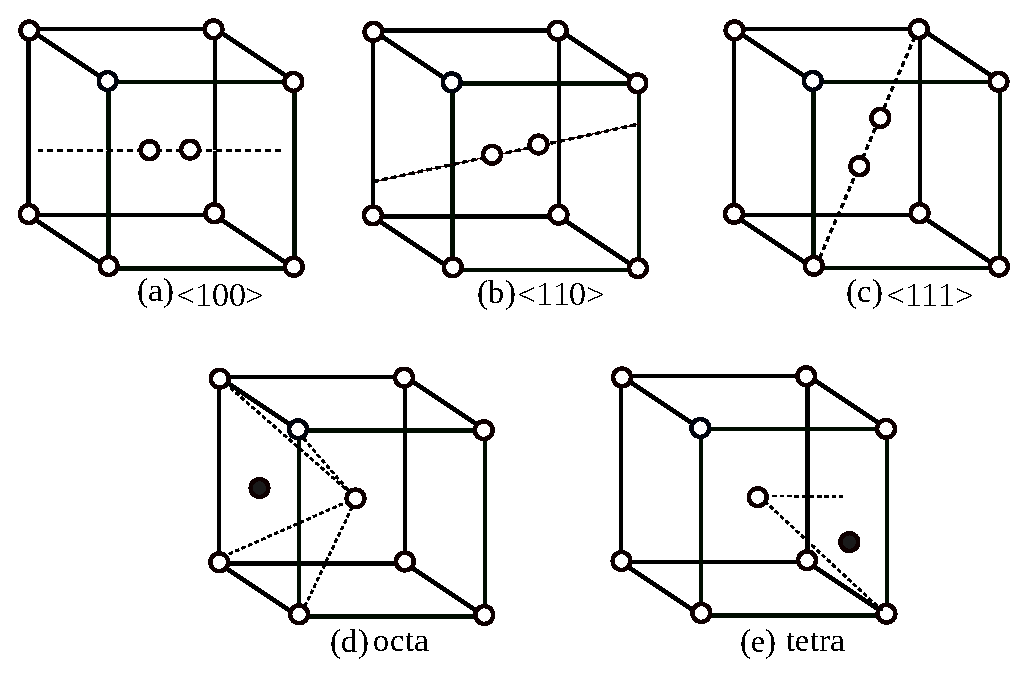
\includegraphics[scale=0.7]{dumbl_figs}
\caption[Different dumbbell configuration in bcc lithium]{Different dumbbell configuration in bcc crystal. a) \hkl<100> dumbbell. b) \hkl<110> dumbbell. c) \hkl<111> dumbbell. d) octahedral interstitial. e) tetrahedral interstitial.}
\label{fig:dmbl}
\end{figure}

\begin{figure}
\centering
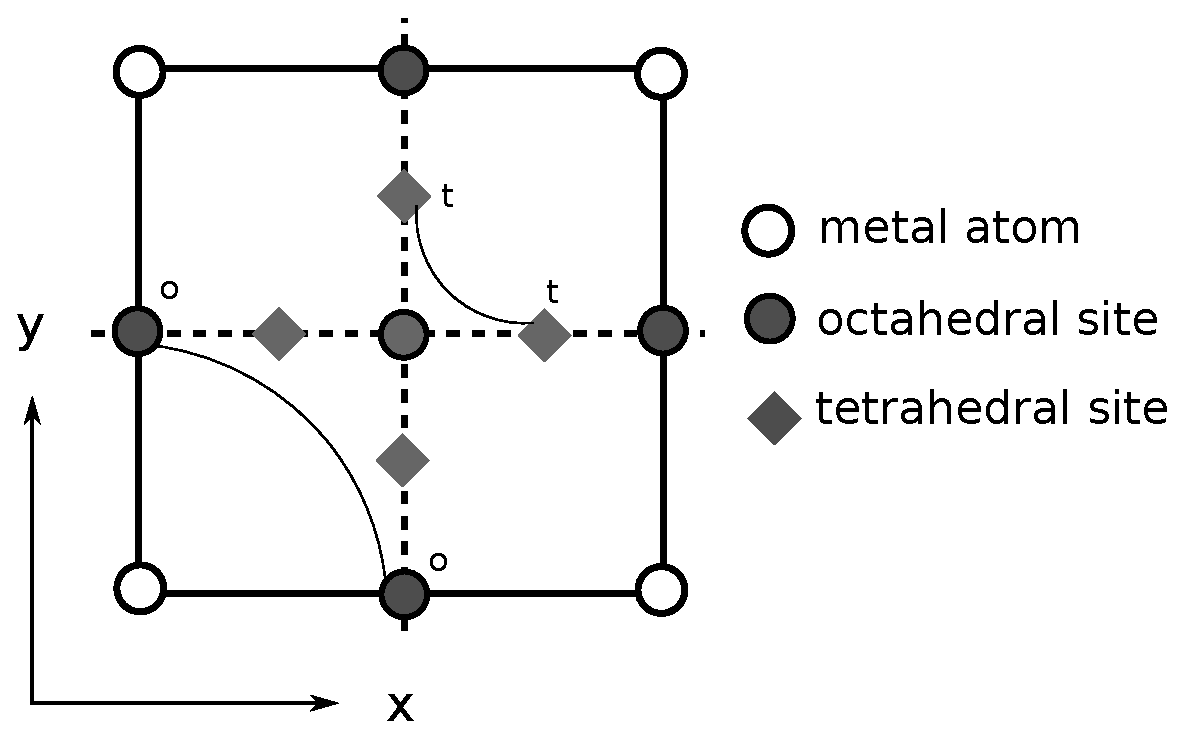
\includegraphics[scale=0.6]{001_oct_tetra}
\caption[Interstitial atom location in 2D for bcc crystal]{Tetrahedral (t) and octahedral (o) site on the (001) plane of the bcc lattice.}
\label{fig:001}
\end{figure}

\begin{figure}
\centering
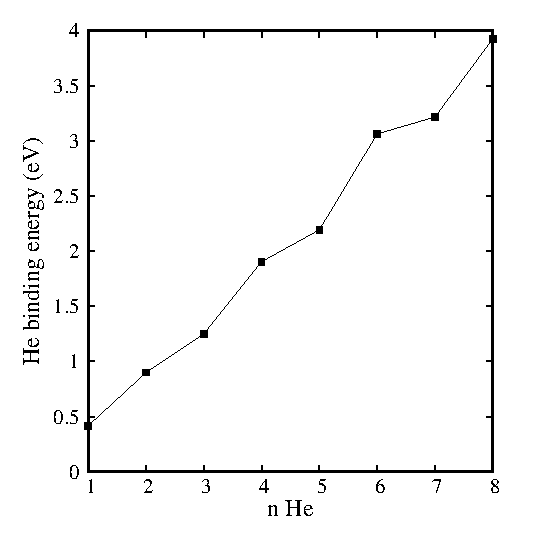
\includegraphics[scale=1.2]{he-vac-bind-E}
\caption[He binding energy]{Helium binding energy around a vacancy}
\label{fig:he-bind}
\end{figure}

\pagebreak
%\bibliographystyle{iopart-num}
\bibliographystyle{apsrev4-1}
\bibliography{abbreviated,lihe}
